\section{Additional Numerical Investigation}
\label{2405:sec:app:numerics}
In this section, we present further numerical investigation to support our theory and extend it beyond the mathematical hypotheses used in the formal proof. 

\subsection{Testing wider range of Algorithm~\ref{2405:algo:optimizer_main_step}}
In the main we presented all the numerical simulation using \(\rho>0\), i.e. \emph{ExtraGradient method/descent}. 
In Figure~\ref{2405:fig:app:other-algos}~Left, we repeat one of the experiment of Figure~\ref{2405:fig:main:single_index_complete} in the case \(\rho<0\), the \emph{Sharpe Aware Minimization}. The two algorithms are based on very different principle, but in our context they behave in the same way: the reusing of the data makes high information exponent function easily learnable. The global picture for \(\rho\neq0\) is the same regardless of its sign. 

\begin{figure}
    \centering
    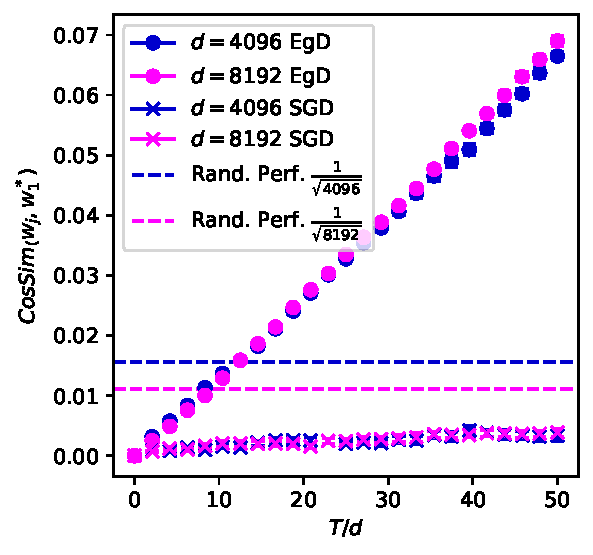
\includegraphics[width=0.4\textwidth]{figs/fig_oa_SAM}
    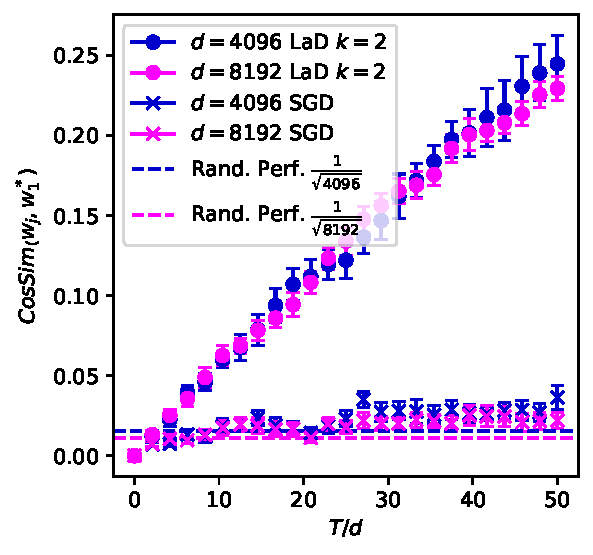
\includegraphics[width=0.4\textwidth]{figs/fig_oa_twosteps}
    \caption{
        example of two different algorithm with data repetitions learning an hard single-index target \(h^\star(\vec z)=\mathrm{He}_3(z_1)\), \(\ell =3, \ell^\star=1\).
        \textbf{Left}: SAM, with \(\rho_0=0.1,\gamma_0=0.01\).
        \textbf{Right}: 2-Lookahed with \(\gamma_0=0.1\).
        See details in App.~\ref{2405:sec:app:implementation}.
    }
    \label{2405:fig:app:other-algos}
\end{figure}
Altought Algorithm~\ref{2405:algo:optimizer_main_step} includes a broad variety of algorithm, it is not the most general domain of validity of our theory. Simple algorithms such as repeating the gradient step twice on the same data before discarding it (also known as \emph{2-lookahead optimizer} \citep{zhang2019lookahead}) are not part of Algorithm~\ref{2405:algo:optimizer_main_step}, yet our considerations are still valid. In fact, the data repetition is sufficient to introduce correlations across two consecutive steps, whose effect builds up along the dynamics causing the network to learn hard targets. A simple illustration of this claim is available in Figure~\ref{2405:fig:app:other-algos}~Right.

\subsection{Extensive batch size}
In this section, we want to present some evidence that our result does not change when the batch size is $1 < n_b \le O(d^{\frac{\ell^\star}{2}})$. The formal proof we presented in the paper is valid in the case where the batch size is \(n_b=1\), but we strongly believe it is the case when training with larger batches.

In the context of the information exponent, it has been shown in \cite{arnaboldi2024online} that the total sample complexity does not change when using batch sizes \(n_b \le O\left(d^{\frac{\ell}{2}}\right)\). The heuristic argument for this behavior is that using a larger batch size increases the learning rate since the noise of the gradient is ``more'' averaged out, ultimately reducing the number of steps.
The same argument should pass from information exponent to generative exponent, allowing the claim (when \(n_b \le O\left(d^{\frac{\ell^\star}{2}}\right)\)) 
\begin{align}
    T \cdot n_b \sim 
        \begin{cases}
        &O(d^{\ell -1} ) \qquad \text{if $\ell^\star>2$} \\
        &O(d \log{d} ) \qquad \text{if $\ell^\star=2$} \\
        &O(d) \qquad \text{if $\ell^\star=1$}
    \end{cases}.
\end{align}

Note that this drastically reduces the time steps needed to learn the teacher's directions, although the sample complexity does not change. \cite{dandi2024benefits} first shows that some high-information exponent functions, such as \(\mathrm{He}_3\), can be learned in just a few steps with full-batch gradient descent \(n_b = O(d)\). In the same work, they introduce a larger class of hard functions that cannot be recovered in \(T=O(1)\), not providing any information on possible bounds on the number of time steps, nor any claim suggesting that not all the function in the class have the same sample complexity. Our theory can provide a full understanding of the phenomena:
\begin{itemize}
    \item \(\mathrm{He}_3\) has generative exponent \(\ell^\star=1\), that implies we need \(O(d)\) samples to weakly recover the target; when training with batch size \(n_b=O(d)\), we have \(T=O(1)\) as in \cite{dandi2024benefits}; Figure~\ref{2405:fig:app:single-index-large-batch}~(Left) is a numerical proof of this fact.
    \item \(\mathrm{He}_4\) has generative exponent \(\ell^\star=2\), that implies we need \(O(d\log d)\) samples to weakly recover the target; when training with batch size \(n_b=O(d)\), we have \(T=O(\log d)\); Figure~\ref{2405:fig:app:single-index-large-batch}~(Right) is a numerical proof of this fact.
\end{itemize}

\begin{figure}
    \centering
    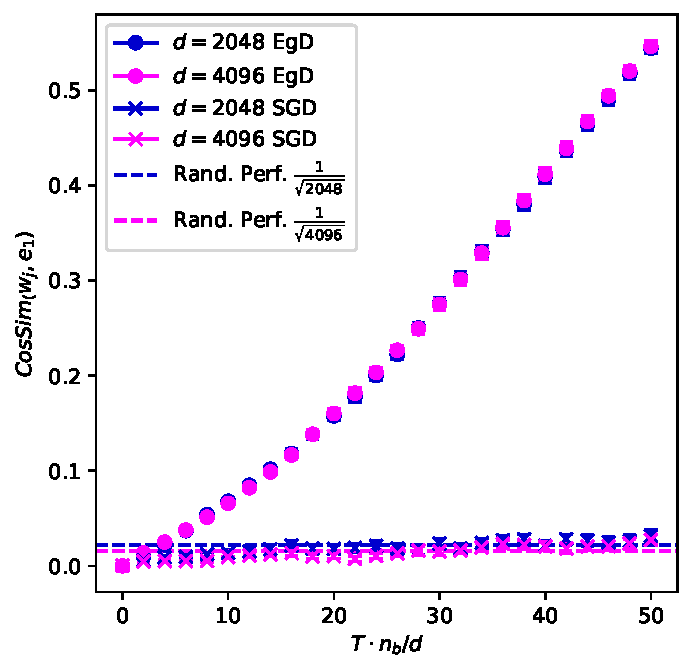
\includegraphics[height=0.4\textwidth]{figs/fig_lb_H3Relu}
    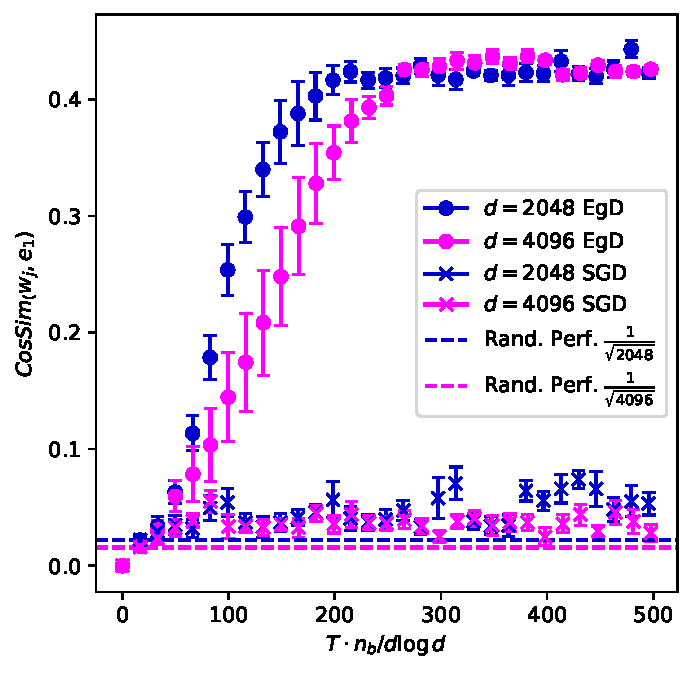
\includegraphics[height=0.4\textwidth]{figs/fig_lb_H4Relu}
    \caption{
        Single-index recovery for large-batch training.
        The dashed horizontal line $\frac{1}{\sqrt{d}}$ is a visual guide to place random performance.
        The plots show $\sigma = \mathrm{relu}$, $\gamma=0.01$, $\rho = 0.1$, and the performance is computed averaging across 10 different runs.
        \textbf{Left $(\ell,\ell^\star)=(3,1)$:} $h^\star = \mathrm{He}_3.$
        \textbf{Right $(\ell,\ell^\star)=(4,2)$:} $h^\star = \mathrm{He}_4$.
        See details in App.~\ref{2405:sec:app:implementation}.
    }
    \label{2405:fig:app:single-index-large-batch}
\end{figure}

We can push our claims beyond single-index targets and illustrate the same phenomena for multi-index functions.
In Figure~\ref{2405:fig:app:multi-index-large-batch} we test Extragradient Descent against two hard multi-index functions: once again the sample complexity is the same as the case \(n_b=1\), while the number of steps is reduced by a factor \(n_b=d\).

\begin{figure}
    \centering
    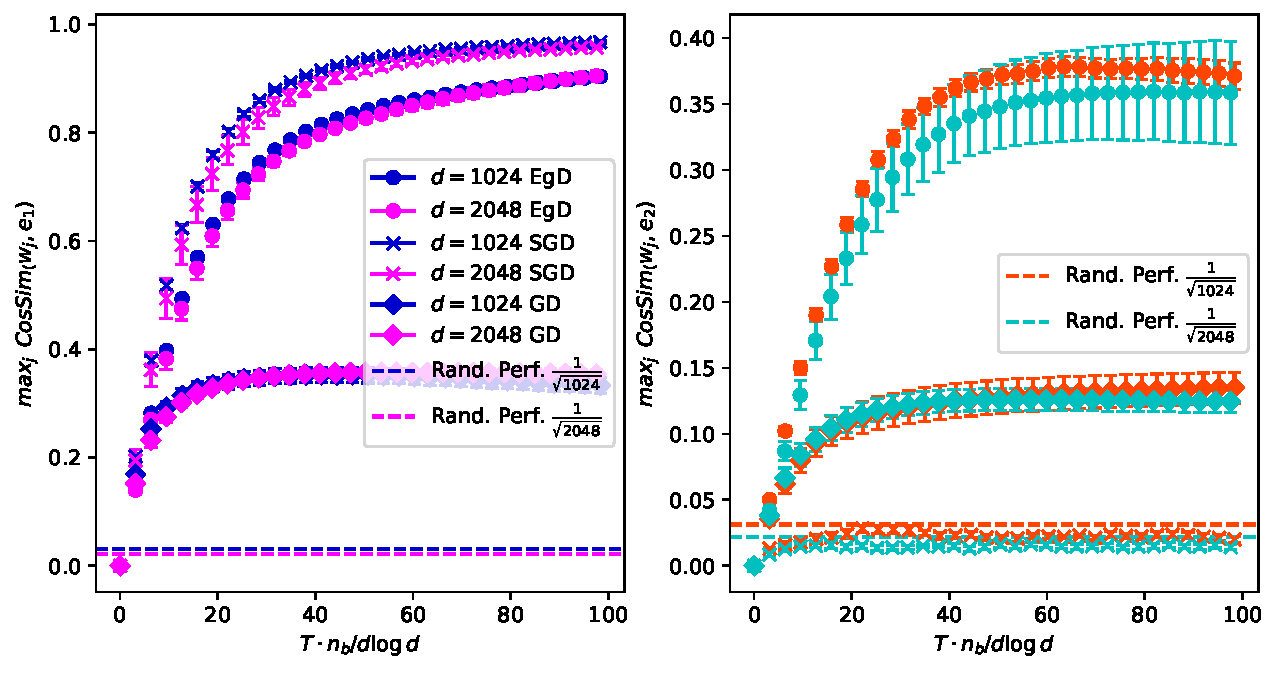
\includegraphics[height=0.45\textwidth]{figs/fig_lb_k3_kstar1}
    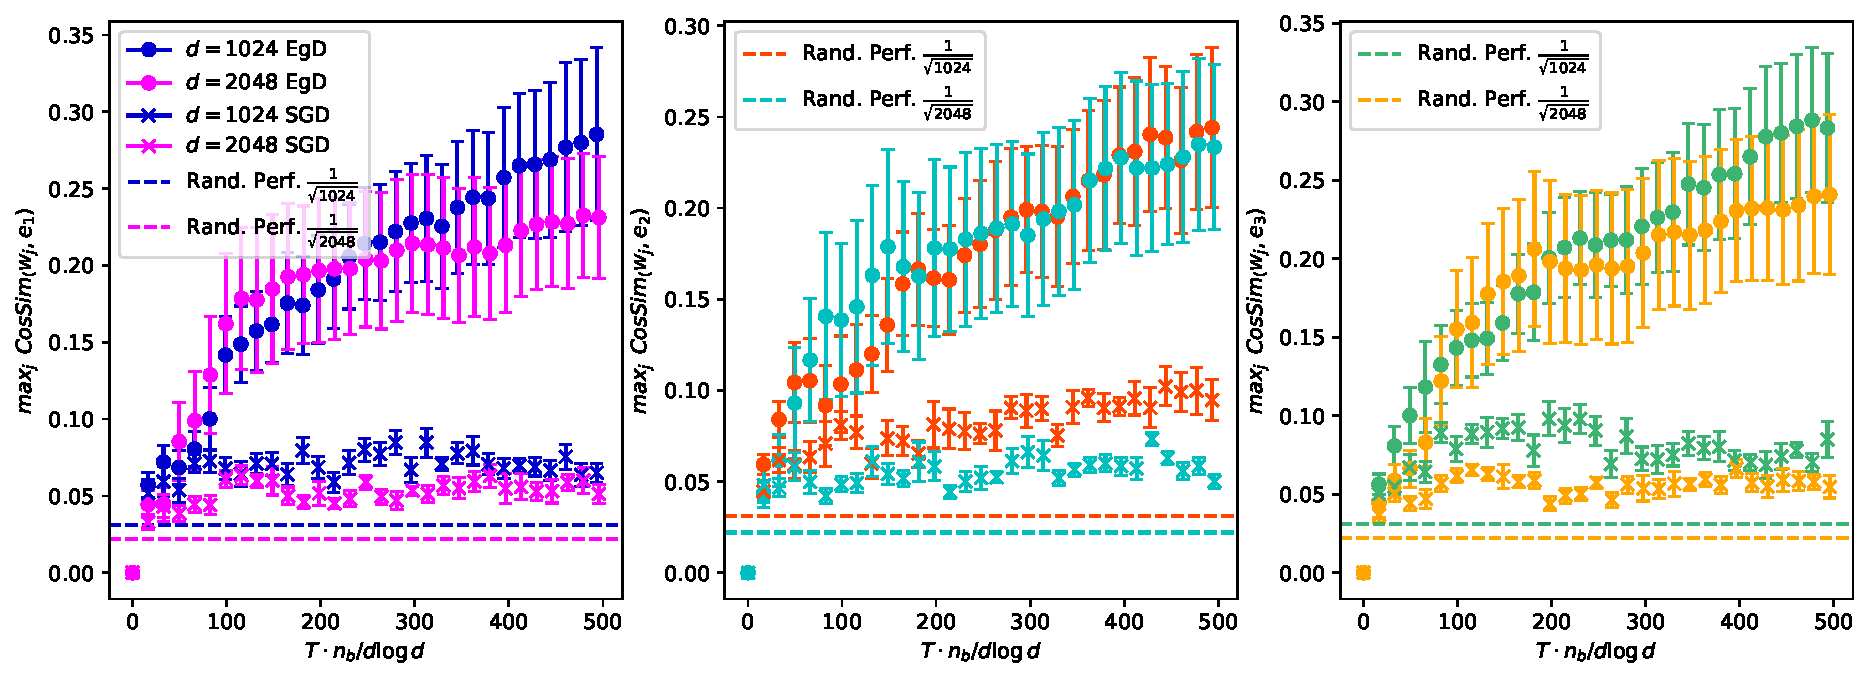
\includegraphics[height=0.33\textwidth]{figs/fig_lb_k3_kstar2}
    \caption{%
        Multi-index recovery for large-batch training.
        The dashed horizontal line $\frac{1}{\sqrt{d}}$ is a visual guide to place random performance.
        The plots show $\sigma = \operatorname{relu}$.
        \textbf{Upper $(\ell_{\vec{v}},\ell_{\vec{v}}^\star)=(3,1)$:} $h^\star(\vec z) = \operatorname{sign}(z_1z_2).$
        \textbf{Lower $(\ell_{\vec{v}},\ell_{\vec{v}}^\star)=(4,2)$:} $h^\star(\vec z) = z_1z_2z_3$.
        See Appendix~\ref{2405:sec:app:implementation} for details.}
    \label{2405:fig:app:multi-index-large-batch}
\end{figure}

% \subsection{Beyond data resuing: numerical investigations}
% Points we have to make here:
% \begin{itemize}
%     \item Changing the loss make hard functions easy, but introduce new hard functions. See Figure~\ref{2405:fig:app:exponential_loss} in order to see an example of hard function for square loss (\(\mathrm{He}_3, \ell = 3\)) that becomes easy learnable for exponential loss.
%     \item Full batch SGD is yet another way to introduce correlations that ultimately allow learning, as presented in \cite{dandi2024benefits}. See Figure~\ref{2405:fig:app:multi-index-large-batch}~Upper for an example.
% \end{itemize}
% \begin{figure}
%     \centering
%     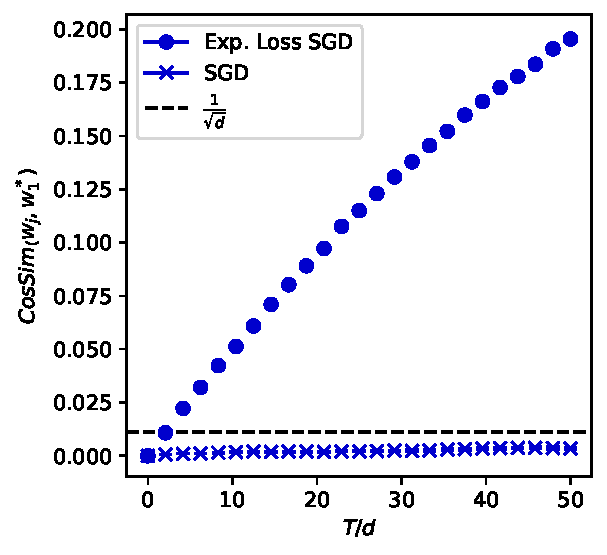
\includegraphics[height=0.33\textwidth]{figs/fig_exponential}
%     \caption{Exponential loss vs square loss SGD.}
%     \label{2405:fig:app:exponential_loss}
% \end{figure}

% \subsection{An example of SQ-Staircase function}
% As we discussed in the main, the introduction generative exponent for multi-index model unveil a new type of stair mechanism, playing the same role as the information exponent in \cite{abbe2021staircase}. We refer to the latter as \emph{CSQ-staircase} targets, while we informally call the new class we are presenting \emph{SQ-staircase functions}. 

% The plot in Figure~\ref{2405:fig:main:staircase} is showing the staircase mechanism in action for a target that is both \emph{SQ-staircase} and \emph{CSQ-staircase}.
% Here, we push forward showing the same for the target \(h^\star(\vec z) = \mathrm{He}_4(z_1) + 5\mathrm{sign}(z_1z_2z_3)\), in Figure~\ref{2405:fig:app:csq-staircase}. The information exponent of \(h^\star\) is \(\ell=3\): the three direction \(w^\star_1, w^\star_2, w^\star_3\) are all equally hard and they are learned all together with \(O(d^2)\) samples; the present of the addend \(\mathrm{He}_4\) does not change the hardness of the target since it has information exponent = 4 if considered alone.
% On the other end, the generative exponent of \(h^\star\) is 2, so the direction \(w^\star_1\) can be learned in \(O(d\log d)\) steps, and then helping learn \(w^\star_2, w^\star_3\) in another \(O(d\log d)\) steps. Figure~\ref{2405:fig:app:csq-staircase} clearly shows that at first only the first direction is learned, and only after that also the other two can be weakly correlated.
% \begin{figure}
%     \centering
%     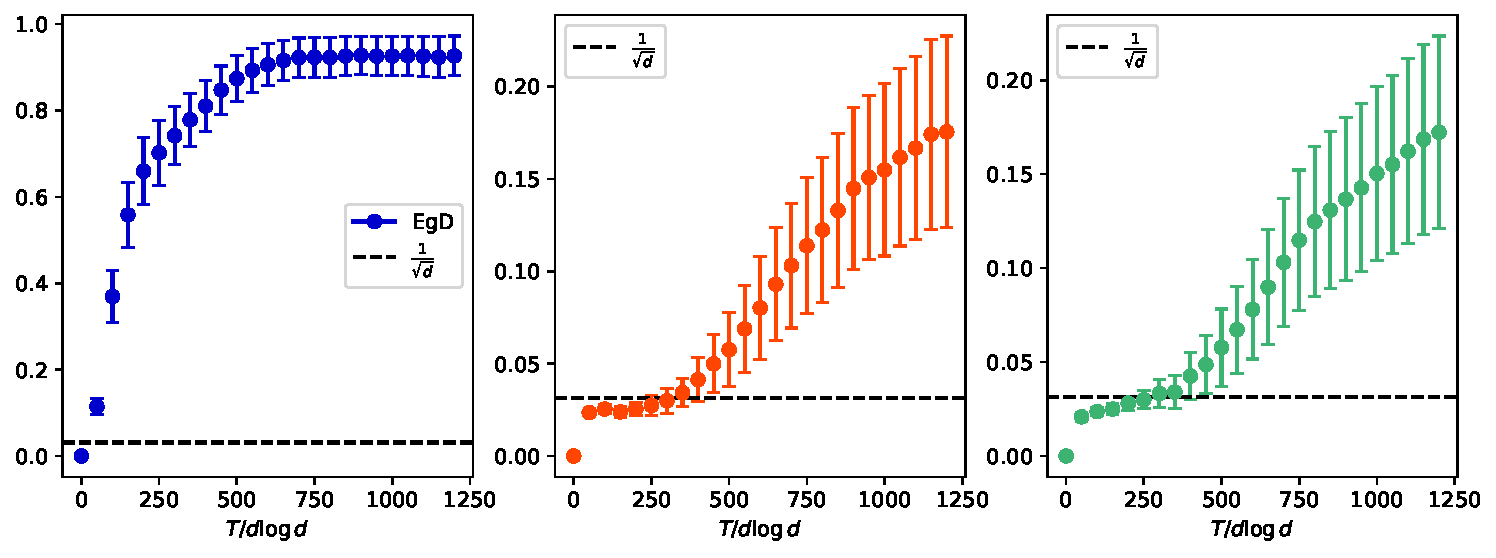
\includegraphics[width=0.8\textwidth]{figs/figs_SQStairH4_long}
%     \caption{learning dynamic of the three hidden direction of the SQ-staircase function \(h^\star(\vec z) = \mathrm{He}_4(z_1) + 5\mathrm{sign}(z_1z_2z_3)\), that is not CSQ-staircase. \(\gamma_0=0.01\), \(\rho_0=0.1\), \(d=1024\), \(\sigma = \mathrm{ReLU}\). See details in App.~\ref{2405:sec:app:implementation}}
%     \label{2405:fig:app:csq-staircase}
% \end{figure}
